\documentclass[12pt, titlepage]{report}
\usepackage{consumer_resource_final}
\graphicspath{{./figures/}}

\begin{document}
% \subsection{Time evolution}
% \begin{figure}[h!]
% \centering
% 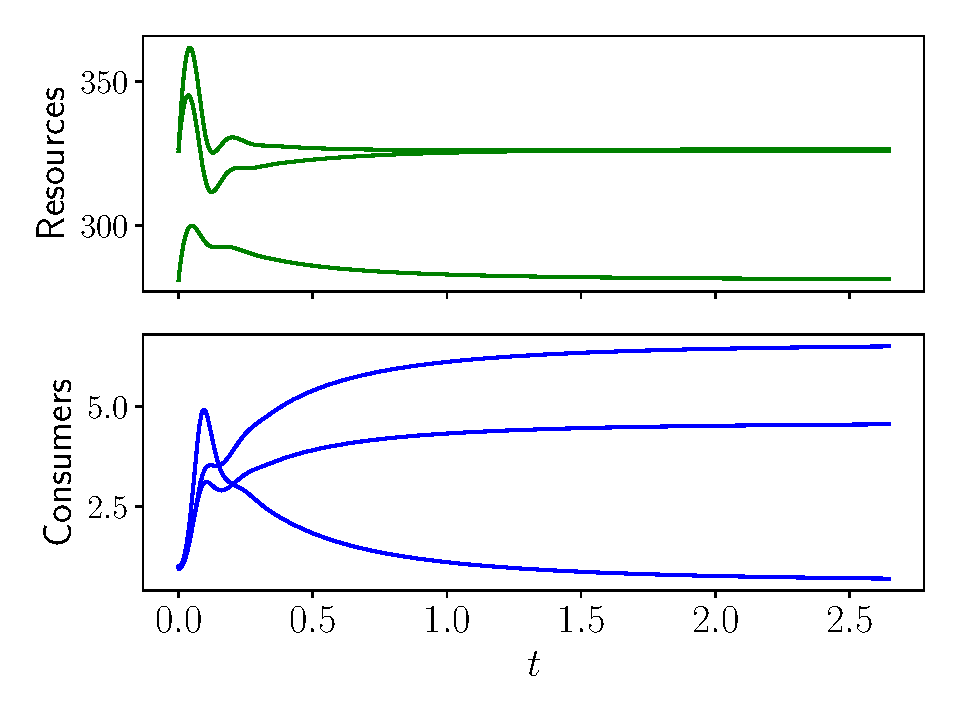
\includegraphics[width=0.6\linewidth]{Typical_time_evolution/Typical_time_evolution_resources_species_high_threshold.pdf}
% \caption{Time evolution for high coefficient threshold ($\epsilon_{\text{conv}}=10^{-1}$)}
% 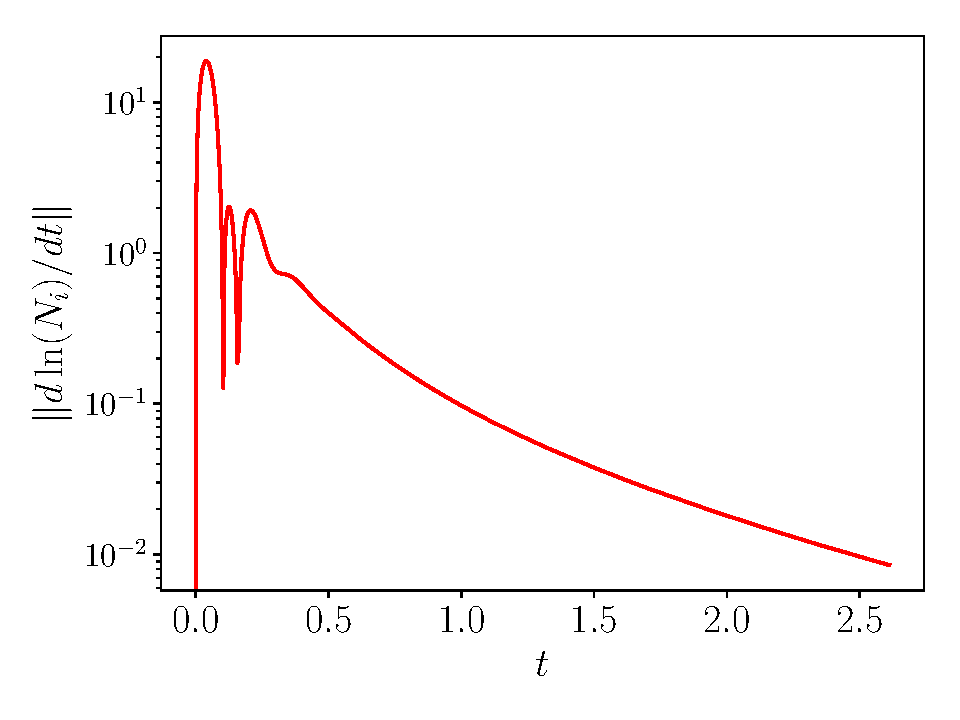
\includegraphics[width=0.6\linewidth]{figures/Typical_time_evolution/Typical_time_evolution_log_derivative_high_threshold.pdf}
% \caption{Typical convergence to judge equilibrium, we see the simulation stops at $\epsilon_{\text{conv}}=10^{-1}$}
% \end{figure}
% \begin{figure}[h!]
% \centering
% 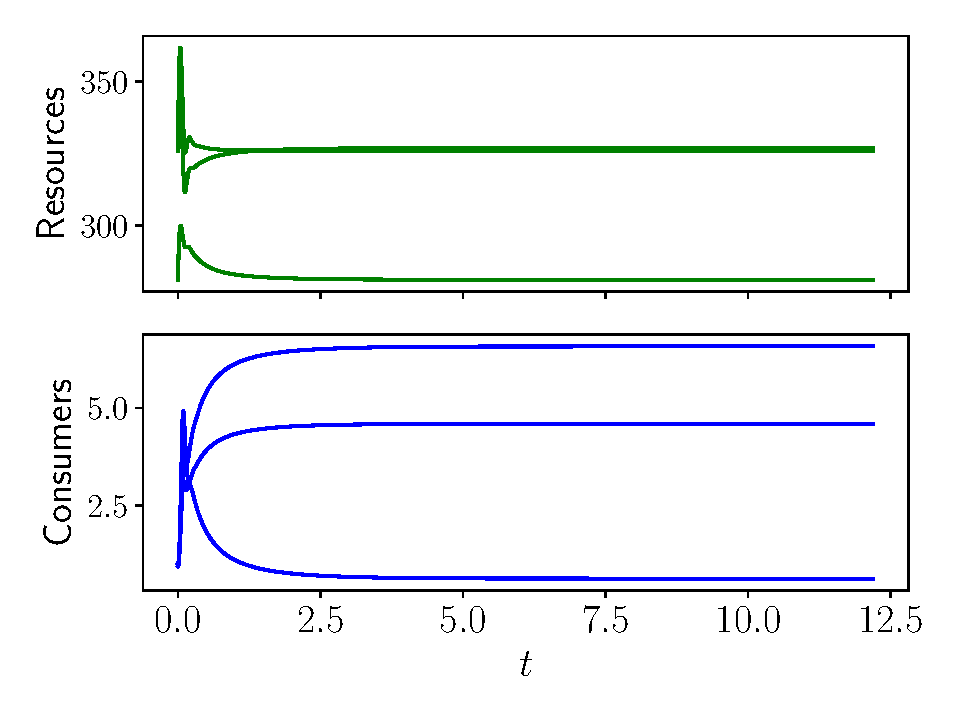
\includegraphics[width=0.6\linewidth]{Typical_time_evolution/Typical_time_evolution_resources_species_low_threshold.pdf}
% \caption{Time evolution for low coefficient threshold (more accuracy) ($\epsilon_{\text{conv}}=10^{-5}$)}
% 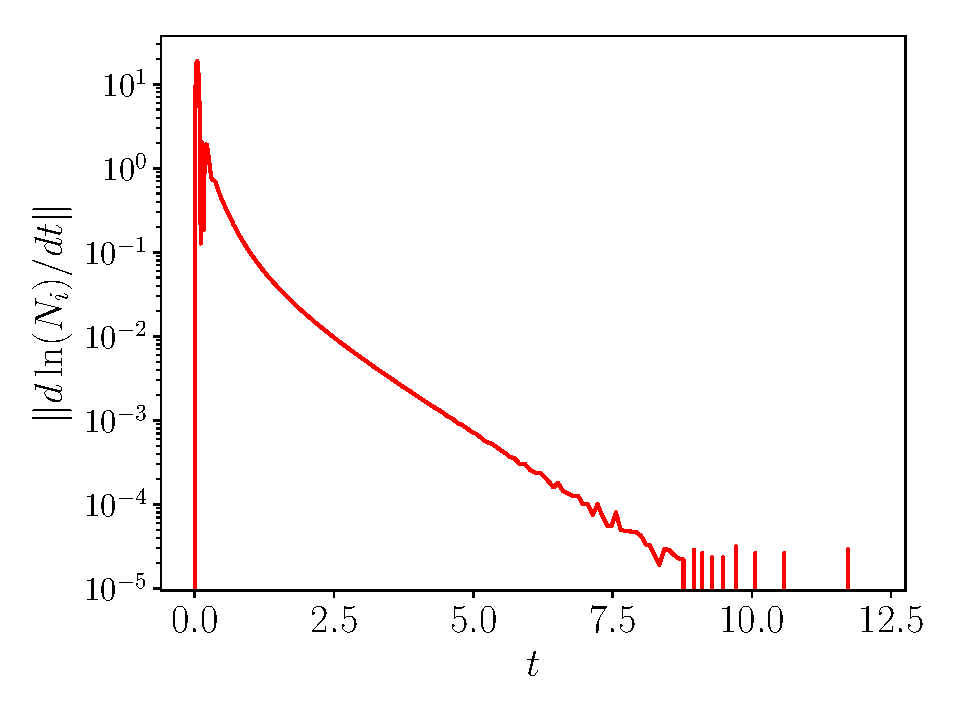
\includegraphics[width=0.6\linewidth]{figures/Typical_time_evolution/Typical_time_evolution_log_derivative_low_threshold.pdf}
% \caption{Typical convergence to judge equilibrium, we see the simulation stops at $\epsilon_{\text{conv}}=10^{-5}$}
% \end{figure}
% \subsection{Allowed parameters : syntrophy range}
% \begin{figure}[h!]
% \centering
% 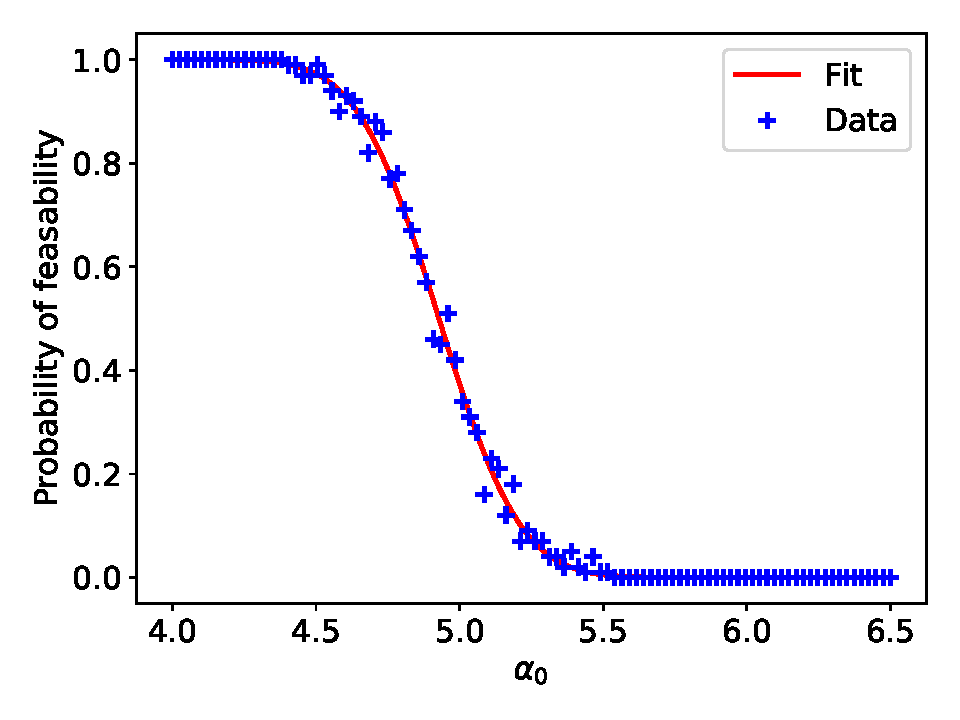
\includegraphics[scale=0.7]{figures/alpha0_probability_of_feasability}
% \caption{Typical shape of the probability of feasability for every metaparameter fixed except varying $\alpha_0$. We see that the probability of drawing a feasible system decreases sharply as $\alpha_0$ increases. A typical sigmoidal curve (here an erf function) fits the numerical data quite well.}
% \end{figure}

% \subsection{Studying the impact of the food network structure}
% \subsection{Studying the impact of syntrophy}
% We run a bunch of simulations with the following metaparameters. We made sure that these are compatible with the bounds on $\alpha_0$ Eqs.\eqref{eq : alpha bounds}.
%
% % Please add the following required packages to your document preamble:
% % \usepackage{graphicx}
% \begin{table}[h!]
% \centering
% \begin{tabular}{c|c|c|c|c|c}
% $\gamma_0$ & $\sigma_0$ & $\alpha_0$ & $R_0$ & $S_0$ & $l_0$ \\ \hline
% 1          & 1          & 0          & 300   & 1     & 11091 \\
%          & 0.75       & 0          &       &       &       \\
%          &            & 0.5        &       &       &       \\
%          & 0.5        & 0          &       &       &       \\
%          &            & 0.5        &       &       &       \\
%          &            & 1          &       &       &       \\
%          & 0.25       & 0          &       &       &       \\
%          &            & 0.5        &       &       &       \\
%          &            & 1          &       &       &       \\
%          &            & 1.5        &       &       &
% \end{tabular}
% \caption{Metaparameters used for the simulations.} \label{eq : table metaparameters used}
% \end{table}

\subsection{LRI regime -- Outcome of the Monte Carlo algorithm}
\begin{figure}
\captionsetup[subfigure]{captionskip = -180pt, margin = 42pt}
\hspace{-0.1\linewidth}
\subfloat[]{\includegraphics[width=0.6\linewidth]{{structure_alpha_matrix_NR25_NS25_with_nestedness}.pdf}}
\subfloat[]{\includegraphics[width=0.6\linewidth]{{structure_alpha_matrix_NR25_N25_with_connectance}.pdf}}

\hspace{-0.1\linewidth}
\subfloat[]{\includegraphics[width=0.6\linewidth]{{structure_alpha_matrix_NR50_NS25_with_nestedness}.pdf}}
\subfloat[]{\includegraphics[width=0.6\linewidth]{{structure_alpha_matrix_NR50_N25_with_connectance}.pdf}}
\end{figure}

\subsection{Fully dynamically stable volume}
\begin{figure}
\captionsetup[subfigure]{captionskip = -230pt, margin = 50pt}
\vspace{-96pt}
\hspace{-0.1\linewidth}
\subfloat[]{\includegraphics[width=1.2\linewidth]{{feasibility_vs_lds_NR25_NS25_Nest0.1_Conn0.1296}.pdf}}

\hspace{-0.1\linewidth}
\subfloat[]{\includegraphics[width=1.2\linewidth]{{feasibility_vs_lds_NR25_NS25_Nest0.6_Conn0.3168}.pdf}}

\caption{Ratio of the size of the fully dynamically stable volume and the fully feasible volume for two consumption matrices $G$ (a) with $\eta_G=0.1$ and $\kappa_G=0.13$, (b) with $\eta_G=0.6$ and $\kappa_G=0.32$. We observe different behaviours for different matrices : for (a) feasibility does not imply local dynamical stability even without syntrophy (it is barely feasible but the ratio is a bit below one for $\alpha_0=0$). On the other hand, for (b) feasibility implies local dynamical stability, indeed both regions have the same volume and since $\mathcal{D}_{L,1}^{G,A}(\alpha_0) \subset \mathcal{F}^{G,A}_1(\alpha_0)$, we conclude that both are equal.}
\end{figure}



\begin{figure}
\captionsetup[subfigure]{captionskip = -185pt, margin = 52pt}
\vspace{-96pt}
\hspace{-0.1\linewidth}
\subfloat[]{\includegraphics[width=1.2\linewidth]{{local_dynamical_stability_wt_wc_region_NR25_NS25_Nest0.35_Conn0.2208}.pdf}}

\vspace{-68pt}
\hspace{-0.1\linewidth}
\subfloat[]{\includegraphics[width=1.2\linewidth]{{local_dynamical_stability_wt_wc_region_NR25_NS25_Nest0.35_Conn0.3216}.pdf}}

\vspace{-68pt}
\hspace{-0.1\linewidth}
\subfloat[]{\includegraphics[width=1.2\linewidth]{{local_dynamical_stability_wt_region_NR25_NS25_Nest0.35_Conn0.272}.pdf}}

\caption{Locally fully dynamically stable region $\mathcal{D}_{L}^{G,1}$ as a function of syntrophy for different matrices $G$. The white zone corresponds to points that are never fully locally dynamically stable. The colour of a given point tells until which syntrophy that point is fully locally dynamically stable, \eg
a green point is fully locally dynamically stable for $0 \leq \alpha_0 \leq \num{6.5e-3}$. Row (a) corresponds to $G$ with $\eta_G = 0.35$ and $\kappa_G = 0.23$, (b) has $\eta_G=0.35$ and $\kappa_G=0.33$ and (c) $\eta_G=0.35$ and $\kappa_G=0.27$. Even at fixed ecological overlap, different connectances of $G$ give rise to completely different systems in terms of local dynamical stability.}
\end{figure}

\begin{figure}
\captionsetup[subfigure]{captionskip = -185pt, margin = 52pt}
\vspace{-84pt}
\hspace{-0.1\linewidth}
\subfloat[]{\includegraphics[width=0.6\linewidth]{{largest_eigenvalue_NR25_NS25_critical_alpha0_fixed_connectance_random_structure}.pdf}}
\subfloat[]{\includegraphics[width=0.6\linewidth]{{largest_eigenvalue_NR25_NS25_critical_alpha0_fixed_nestedness_random_structure}.pdf}}

\vspace{-12pt}
\hspace{-0.1\linewidth}
\subfloat[]{\includegraphics[width=0.6\linewidth]{{largest_eigenvalue_NR25_NS25_critical_alpha0_fixed_connectance_no_release_when_eat}.pdf}}
\subfloat[]{\includegraphics[width=0.6\linewidth]{{largest_eigenvalue_NR25_NS25_critical_alpha0_fixed_nestedness_no_release_when_eat}.pdf}}

\vspace{-12pt}
\hspace{-0.1\linewidth}
\subfloat[]{\includegraphics[width=0.6\linewidth]{{largest_eigenvalue_NR25_NS25_critical_alpha0_fixed_connectance_optimal_matrix}.pdf}}
\subfloat[]{\includegraphics[width=0.6\linewidth]{{largest_eigenvalue_NR25_NS25_critical_alpha0_fixed_nestedness_optimal_matrix}.pdf}}
\vspace{-12pt}
\caption{Critical syntrophy $\alpha_0^D$, defined as the smallest syntrophy for which we can still find metaparameters that will give rise to fully dynamically stable systems. How $\alpha_0^D$ is estimated is explained in the main text. Errors on $\alpha_0^D$ are not plotted but are at most around $10\%$. (a)(c)(e) Evolution of $\alpha_0^D$ with ecological overlap $\eta$ at different connectance. (b)(d)(f) Evolution of $\alpha_0^D$ with connectance $\kappa$ for different ecological overlap. We observe a strong trend : for a given connectance, $\alpha_0^D$ decreases as ecological overlap increases. Also, for a given ecological overlap, $\alpha_0^D$ increases as connectance is increased.}\label{fig : dynamical stability results critical dynamical syntrophy}
\end{figure}


\subsection{Largest eigenvalue of the jacobian}
Equation \ref{eq : dynamical stability methods fully connected metaparameters} from Methods \ref{sec : methods dynamical stability fully connected zero variance} gives a relationship that the metaparameters should approximately follow in order to give rise to locally dynamically stable systems. Although strictly speaking it is only valid for the case where both $G$ and $A$ are fully connected, we expect it to work as well when $G$ and $A$ are \important{not too far away} from the fully connected case. It tells us that in order to get more local dynamically stable systems you should :
\begin{itemize}
  \item decrease $N_S$, $l_0$ \textbf{WEIRD RESULT : would expect that increasing l0 would make systems more dynamically stable (observed in simulations I think)} or $\alpha_0$,
  \item if $\alpha_0 - \gamma_0 R_0 < 0$, increase $N _R$, $\sigma_0$ and $\gamma_0$,
  \item be careful in how you handle $S_0$ : increasing $S_0$ reduces the $l_0^2/S_0$ term but increases the $N_S^2 \alpha_0^2 S_0$ term. It is very easy to show (Appendix \ref{sec : appendix how to handle S0}) that if $S_0 > l_0/(N_S \alpha_0)$ it should be decreased, and otherwise it should be increased until it reaches $l_0/(N_S \alpha_0)$.
\end{itemize}

Combining these with the feasibility conditions Eq.\eqref{eq : fully feasible volume} we expect that -- for all other metaparameters fixed -- systems get more and more locally dynamically stable as $\gamma_0$ is increased and $S_0$ is the largest possible. In short, points at the upper border of $\mathcal{D}^{G,A}_{L,1}$ should have a lower and lower $\real{\lambda_1}$ as $\gamma_0$ increases. Figure \ref{fig : local dynamical stability results largest eigenvalue} shows that indeed this trend is followed.
\begin{figure}
\vspace{-72pt}
\hspace{-0.0\linewidth}
\subfloat[]{\includegraphics[width=\linewidth]{{largest_eigenvalue_wt_NR25_NS25_Nest0.1_Conn0.1296_alpha0=0.0}.pdf}}

\vspace{-26pt}
\hspace{-0.0\linewidth}
\subfloat[]{\includegraphics[width=\linewidth]{{largest_eigenvalue_wt_NR25_NS25_Nest0.1_Conn0.1296_alpha0=0.0039}.pdf}}

\vspace{-26pt}
\hspace{-0.0\linewidth}
\subfloat[]{\includegraphics[width=\linewidth]{{largest_eigenvalue_wt_NR25_NS25_Nest0.1_Conn0.1296_alpha0=0.0078}.pdf}}
\caption{Largest real eigenvalue $\text{Re}(\lambda_1)$ averaged over 300 realisations for each $(\gamma_0, S_0)$ points for the consumption matrix $G$ with consumers overlap $\eta_G = 0.1$ and connectance $\kappa_G=0.13$. The white points correspond to not fully dynamically stable systems. Each row corresponds to a different syntrophy value (a) $\alpha_0 = 0$ (no syntrophic interaction), (b) $\alpha_0 = \num{3.9e-3}$ and (c) $\alpha_0 = \num{7.8e-3}$. The first column corresponds to the regime where $A$ is fully connected, the second where $A$ forbids intraspecific syntrophy and the third is the outcome of the MC algorithm. As syntrophy increases, the size of the fully dynamically stable region decreases. Furthermore, the boundary points close to the $\gamma_0 \sim S_0^{-1}$ curve are the most stable in every situation.}\label{fig : local dynamical stability results largest eigenvalue}
\end{figure}
This tells us that if we keep the consumption flux $N_S \gamma_0 S_0$ constant, increasing $\gamma_0$ (and hence decreasing $S_0$) will give rise to more stable systems. Notice that contrarily to the prediction made above, increasing $\alpha_0$ does not decrease stability but increases the maximal $\abs{\real{\lambda_1}}$ observed as shows Fig.\ref{fig : dynamical stability results typical maximal eigenvalue observed varying syntrophy}. This is coupled with the shrinkage of the fully locally dynamically stable volume seen on Fig.\ref{fig : dynamical stability results shrinkage of DL1G varying syntrophy}. This means that overall increasing syntrophy makes the system \important{more stable} but at \important{fewer points}. This hints that systems in a high syntrophic regime, where consumers produce a lot of resources, should be very fine-tuned and occur for very specific consumption strength and average abundance of consumers.
\begin{figure}
\hspace{-0.1\linewidth}
\captionsetup[subfigure]{captionskip = -210pt, margin = 26pt}
\subfloat[\label{fig : dynamical stability results typical maximal eigenvalue observed varying syntrophy}]{\includegraphics[width=0.6\linewidth]{{largest_eigenvalue_varying_syntrophy_NR25_NS25_Nest0.3_Conn0.2272}.pdf}}
\subfloat[\label{fig : dynamical stability results shrinkage of DL1G varying syntrophy}]{\includegraphics[width=0.6\linewidth]{{size_local_dynamical_stability_region_NR25_NS25_Nest0.3_Conn0.2272}.pdf}}
\caption{For a consumption matrix $G$ with $\eta_G=0.3$ and $\kappa_G=0.23$. (a) Evolution of the maximal $\abs{\av{\real{\lambda_1}}}$ observed in the $(\gamma_0,S_0) \in [0,1]^2$ region. The maximal eigenvalue increases in magnitude, making the system more dynamically stable, as syntrophy increases. That trend is true for all matrices we considered. (b) Volume of $\mathcal{D}^G_{L,1}(\alpha_0)$. As syntrophy increases, fewer and fewer points become fully dynamically stable. For both figures, the different lines show the different stand for the different structure of the syntrophy matrix that we considered.}
\end{figure}

Coming back to the reasoning above, we expect stability to increase when the number of resources is increased for a fixed number of consumers.




\end{document}
